\subsection*{Devices}

We collected data using a 22-sensors Immersion DataGlove for the hand
posture, an Ascension Flock-Of-Birds (FoB) for the hand position and a
Force Resistor Sensor (FSR) to detect the contact moment with the
object.

The DataGlove was worn by the subject on the right hand. The device
returns $22$ $8$-bit numbers, describing the position of the three
phalanxes of each finger (for the thumb, rotation and two phalanxes),
the four finger-to-finger abductions, the palm arch, the wrist pitch
and the wrist yaw. The FoB sensor was firmly mounted on the DataGlove,
just above the subject's wrist, with the X/Y plane being parallel to
the palm plane in the resting position. The device returns $6$
double-precision numbers describing the position ($x$, $y$ and $z$ in
inches) and rotation (azimuth, elevation and roll in angles) of the
sensor with respect to a magnetic basis mounted about one meter away
from the subject. The FSR was mounted on the subject's thumb. It
returns a $32$-bit number approximately inversely proportional to the
pressure applied to the surface of the sensor. All devices were tuned
to stream at $100$Hz, and their data were synchronised, collected and
saved in real time. Figure \ref{fig:devices} shows the devices, as
worn by a subject.

\begin{figure}[htbp]
  \begin{center}
    \begin{tabular}{cc}
      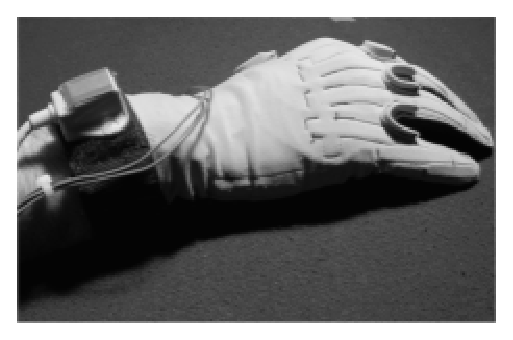
\includegraphics[width=0.45\linewidth]{devices1.eps} &
      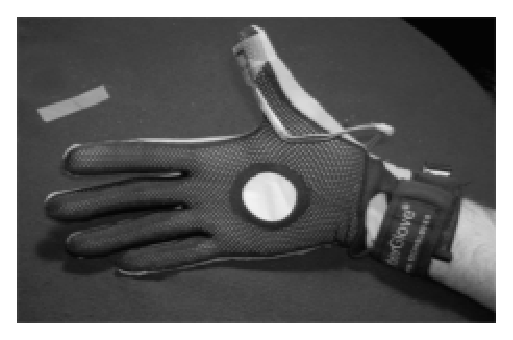
\includegraphics[width=0.45\linewidth]{devices2.eps} \\
      $(a)$ & $(b)$
    \end{tabular}
    \caption{The devices used for the experiment, as worn by a
    subject: $(a)$ the DataGlove with the Flock-of-Birds just above the
    subject's wrist; $(b)$ the Force Resistor Sensor attached to the
    subject's thumb.}
    \label{fig:devices}
  \end{center}
\end{figure}

\subsection*{Subjects}

Eleven subjects, four females and seven males aged $24$ to $34$ of
several different nationalities, joined the experiment. They were all
right-handed and fully able-bodied, and were given initially some
knowledge of the aim of the experiment.

\subsection*{Experimental setup}

The subjects were asked to sit confortably in front of a clean
workspace of about one squared meter, at the center of which an object
was placed, in a predefined position. The subjects were then asked to
wear the DataGlove (along with the FoB and FSR), and to choose a
resting position for their right hand and arm.

The subjects had to grasp the object with their right hand any way
they wanted, not necessarily the same way each time, keeping a
``natural'' attitude, i.e., without employing weird hand positions
and/or postures, but being able to seize the object with precision or
power grips, using the whole hand cilyndrically or just a subset of
their fingers, etc. After grasping the object, they had to drop it
somewhere else in the workspace, and then return their right hand and
arm in the initial resting position. Subsequently, they had to use
their left hand to reposition the object roughly in the same place it
was before.

We first had the subjects do a trial run of the experiment, in order
for them to gain confidence in the setup. A beeping sound was heard
each time the subject made contact with the object (that is, each time
the FSR signalled a significant change), and they were asked to try
and hear the beep each time they grasped the object. Although this
ruled out grasps which made no use of the thumb, it enabled us to
better understand the contact point.

After the trial run, subjects were asked to repeat the
grasp/drop/reposition procedure $120$ times per each object. We
employed, in turn, three objects: a beer can, a scotch tape roll and a
mug (Figure \ref{fig:objects} shows the objects).

\begin{figure}[htbp]
  \begin{center}
    \begin{tabular}{ccc}
      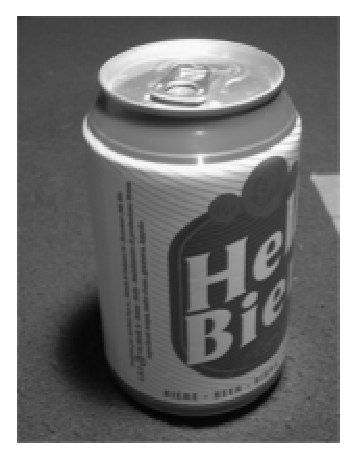
\includegraphics[width=0.3\linewidth]{beer.eps} &
      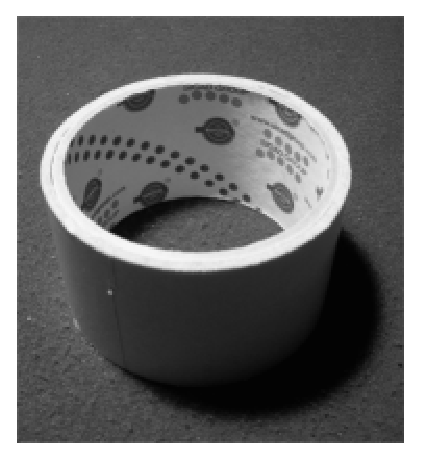
\includegraphics[width=0.3\linewidth]{scotch.eps}  &
      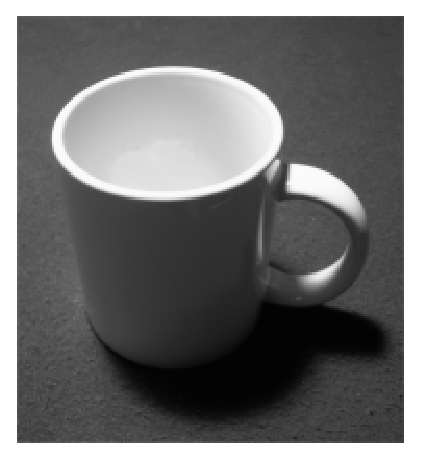
\includegraphics[width=0.3\linewidth]{mug.eps} \\
      $(a)$ & $(b)$ & $(c)$
    \end{tabular}
    \caption{The objects used inthe experiment: a beer can $(a)$, a scotch
    tape roll $(b)$ and a mug $(c)$.}
    \label{fig:objects}
  \end{center}
\end{figure}

The $120$-grasps session was done twice, resulting in approximately
$240$ grasps for each of the three objects. In order not to have the
subjects ``specialise'' on a particular object, we alternated the
sessions this way: first the can, then the roll and then the mug, all
of this two times.

Experiments lasted $35$ to $56$ minutes depending on the subject's
confidence and speed; although almost no subjects reported tiredness,
we allowed for rest between each session. It was reported by almost
every subject that the experiment became rapidly boring, which lets us
claim that almost all grasps were done in a natural, almost
unconscious way. Figure \ref{fig:setup} shows the main phases of the
experiment.

\begin{figure}[htbp]
  \begin{center}
    \begin{tabular}{ccc}
      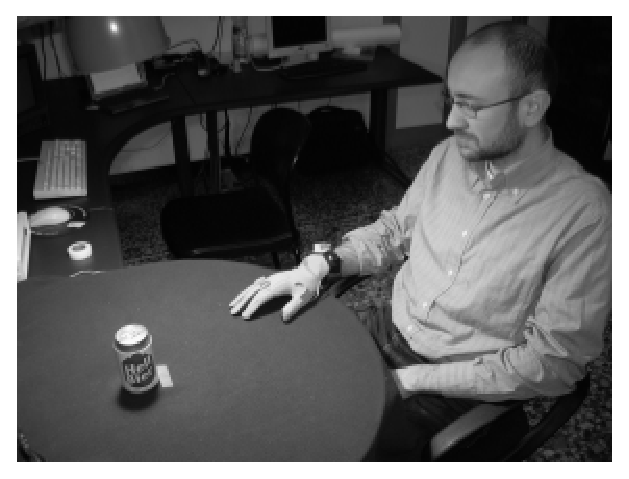
\includegraphics[width=0.3\linewidth]{exp1.eps} &
      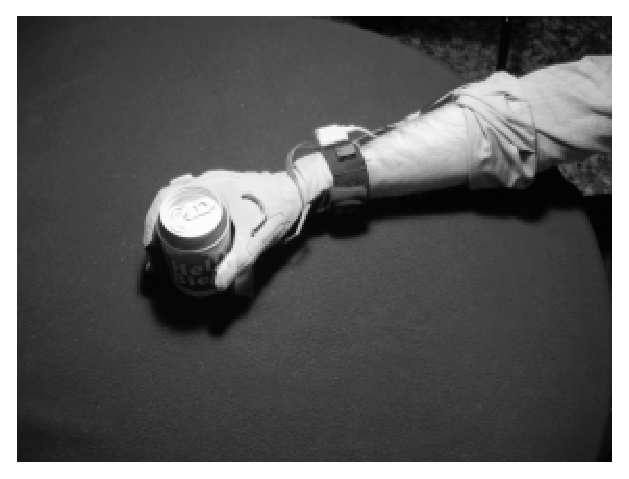
\includegraphics[width=0.3\linewidth]{exp2.eps}  &
      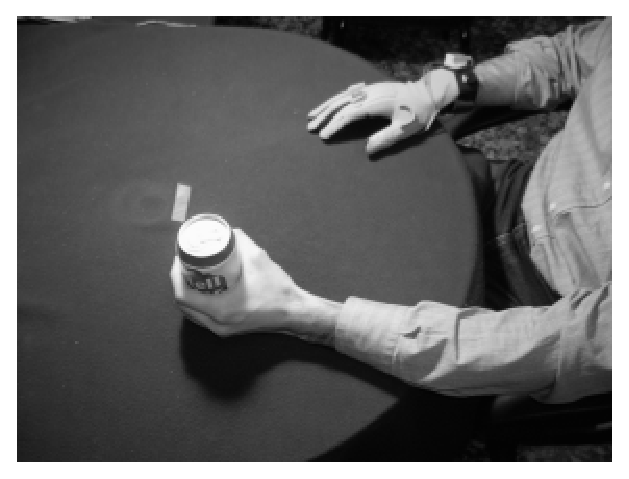
\includegraphics[width=0.3\linewidth]{exp3.eps} \\
      $(a)$ & $(b)$ & $(c)$
    \end{tabular}
    \caption{The experiment. The subject sits confortably in
    front of a clean workspace, at the center of which an object is
    placed $(a)$, with his right hand in a resting position. He then
    grasps the object and drops it somewhere else in the workspace
    $(b)$, bringing then his arm and hand in the resting
    position. Lastly, he repositions the object in the initial
    position using his left arm and hand $(c)$. The procedure is repeated
    for $120$ times, then this session is repeated for each of the
    three objects, and all of this is done twice, resulting in
    approximately $240$ grasps for each subject and object.}
    \label{fig:setup}
  \end{center}
\end{figure}

\subsection*{Data Analysis and Pre-processing}
